\documentclass{amsart}
\usepackage{amsmath,amssymb,stmaryrd,pxfonts,lmodern,tikz}
\usetikzlibrary{external}

\newtheorem{prop}{Proposition}

\newcommand{\id}{\mathrm{id}}
\newcommand{\op}{\mathrm{op}}
\newcommand{\Ob}{\operatorname{Ob}}
\newcommand{\Arr}{\operatorname{Arr}}
\newcommand{\prof}{\multimapdotbothA}
\newcommand{\backref}{\vcenter{\hbox{\larger[2]$\star$}}}
\newcommand{\place}{-}
\newcommand{\base}{\mathrm{base}}
\newcommand{\transformto}{\to}
\newcommand{\canoniso}{=}
\newcommand{\posof}{\in}
\newcommand{\sub}{\mathrel{\triangleleft}}
\newcommand{\subd}{\mathrel{\!\vcenter{\hbox{\larger[-12]$\blacktriangleleft$}}\!}}
\newcommand{\idsub}{\id_{\sub}}
\newcommand{\idsubd}{\id_{\subd}}

\newcommand{\cat}[1]{\mathcal{#1}}
\newcommand{\bundle}[1]{\overset{#1}{\to}}
\newcommand{\shrink}[2][.65]{\scalebox{#1}{$#2$}}
\newcommand{\pos}[1]{#1(1)}
\newcommand{\dir}[2]{#1[#2]}
\newcommand{\posmap}[2]{{#1}_1(#2)}
% \newcommand{\dirmap}[3]{{#1}^\sharp(#2,#3)}
\newcommand{\dirmap}[3]{{#1}^\sharp_{#2}(#3)}
% \newcommand{\anydirmap}[2]{\dirmap{#1}{\place}{#2}}
\newcommand{\anydirmap}[2]{{#1}^\sharp(#2)}

\newcommand{\catname}[1]{{\normalfont\mathbf{#1}}}
\newcommand{\Set}{\catname{Set}}


\definecolor{rcol}{RGB}{255,0,0}
\definecolor{gcol}{RGB}{0,150,0}
\definecolor{pcol}{RGB}{170,0,170}
\definecolor{bcol}{RGB}{0,0,255}
\definecolor{ycol}{RGB}{210,130,0}

\tikzset{every picture/.style={scale=.1,baseline}}

\tikzset{vertex/.style={circle,draw,inner sep=1pt,minimum size=6,text=black}}
\tikzset{edge/.style={-stealth}}
\tikzset{label/.style={rectangle,rounded corners,fill=white,inner
sep=1pt,text=black}}

\tikzset{annot/.style={font=\scriptsize}}
\tikzset{dash/.style={dashed,draw opacity=0.5}}
\tikzset{transparent/.style={draw opacity=0.3,fill opacity=0.3}}
\tikzset{small/.style={minimum size=3.5}}
\tikzset{large/.style={minimum size=12}}
\tikzset{huge/.style={minimum size=17}}
\tikzset{huger/.style={minimum size=27}}
\title{Polynomial comonoids and bicomodules}
\begin{document}
\maketitle

\iffalse
  A \emph{polynomial}\footnote{The name refers to a correspondence
    between families of sets and sums of powers, illustrated by the
    example
    ${2y^4 + y^2 + y \leftrightarrow
      \{\{\ast,\ast,\ast,\ast\},\{\ast,\ast,\ast,\ast\},\{\ast,\ast\},
      \{\ast\}\}}$.} is an indexed family of sets.

  The indexes of sets are called \emph{positions}, and the members of
  indexed sets are called \emph{directions}.

  We will visualize a polynomial as a collection of corollas.

  % figure

  A corolla is a node with arrows pointing out from it; this denotes a
  position and the directions from it.
\fi

Recall the \emph{substitution product} of polynomials $P$ and $Q$, denoted
$P \sub Q$.

\iffalse
  From polynomials $P$ and $Q$, we can form a new polynomial
  of all the possible two-story trees built by stacking $Q$
  corollas atop a $P$ corolla. This is called the \emph{substitution
    product}, denoted $P \sub Q$.
\fi

\begin{itemize}
\item A position $a$ in $P \sub Q$ consists of a position $a_\base$ in
  $P$ and positions $a_f$ in $Q$ for each direction $f$ from
  $a_\base$.
\item A direction from position $a$ in $P \sub Q$ consists of a
  direction $f$ from $a_\base$ and a direction $g$ from $a_f$.
\end{itemize}
\vspace{.5em}
\begin{center}
  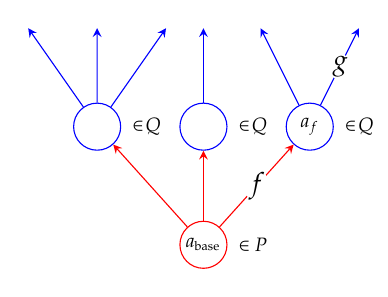
\begin{tikzpicture}
\node [rcol,vertex,huge] (s) at (0, -12) {\scriptsize$a_{\shrink{\base}}$};
\node [bcol,vertex,huge] (m1) at (-13.5,3) {};
\node [bcol,vertex,huge] (m2) at (0,3) {};
\node [bcol,vertex,huge] (m3) at (13.5,3) {\scriptsize$a_f$};
\coordinate (t11) at (-22.25,15.5) {};
\coordinate (t12) at (-13.5,15.5) {};
\coordinate (t13) at (-4.75,15.5) {};
\coordinate (t21) at (0,15.5) {};
\coordinate (t31) at (7.25,15.5) {};
\coordinate (t32) at (19.75,15.5) {};
\draw [rcol,edge] (s) -- (m1);
\draw [rcol,edge] (s) -- (m2);
\draw [rcol,edge] (s) -- node [label] {$f$} (m3);
\draw [bcol,edge] (m1) -- (t11);
\draw [bcol,edge] (m1) -- (t12);
\draw [bcol,edge] (m1) -- (t13);
\draw [bcol,edge] (m2) -- (t21);
\draw [bcol,edge] (m3) -- (t31);
\draw [bcol,edge] (m3) -- node [label] {$g$} (t32);

\node [annot] at (4.5, -12) {\rlap{$\posof P$}};

\node [annot] at (-9, 3) {\rlap{$\posof\!Q$}};
\node [annot] at (4.5, 3) {\rlap{$\posof\!Q$}};
\node [annot] at (18, 3) {\rlap{$\posof\!Q$}};
\end{tikzpicture}

  \qquad
  {\Large$=$}
  \quad
  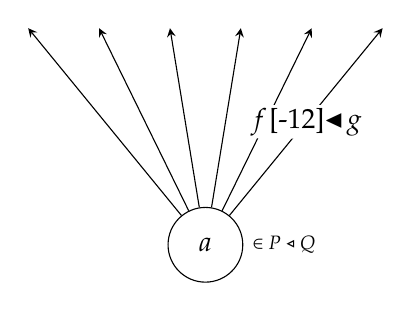
\begin{tikzpicture}
\node [vertex,huger] (s) at (0, -12) {$a$};
\coordinate (t11) at (-22.5,15.5) {};
\coordinate (t12) at (-13.5,15.5) {};
\coordinate (t13) at (-4.5,15.5) {};
\coordinate (t21) at (4.5,15.5) {};
\coordinate (t31) at (13.5,15.5) {};
\coordinate (t32) at (22.5,15.5) {};
\draw [edge] (s) -- (t11);
\draw [edge] (s) -- (t12);
\draw [edge] (s) -- (t13);
\draw [edge] (s) -- (t21);
\draw [edge] (s) -- (t31);
\draw [edge] (s) -- node [label] {$f \subd g$} (t32);

\node [annot] at (6, -12) {\rlap{$\posof P \sub Q$}};
\end{tikzpicture}

\end{center}
\vspace{1em}

We denote such a direction from such a position in a substitution
product by $f \subd g$.\footnote{Be aware there may be other
  directions named $f \subd g$ from other positions in
  $P \sub Q$.} Accordingly, $\idsubd$ will denote the unique direction
from the unique position in the unit for substitution $\idsub$
(a.k.a. the polynomial $y$).\iffalse\footnote{Given directions $f$,
    $g$, and $h$ respectively belonging to polynomials $P$, $Q$, and
    $R$, directions of the form $(f \subd g)\subd h$ belonging to
    $(P \sub Q) \sub R$ and directions of the form
    $f \subd (g \subd h)$ belonging to $P \sub (Q \sub R)$ are
    identified under the relevant monoidal coherence
    isomorphism. Hence brackets can be omitted.

  Similarly, for any direction $f$ belonging to a polynomial $P$, we
  have that $\idsubd \subd f$ and $f \subd \idsubd$ (respectively
  belonging to $\idsub \sub P$ and $P \sub \idsub$) are both
  canonically identified with $f$.}\fi

\iffalse
  Suppose we have polynomials $P$ and $Q$ and the following
  structure relating them.
  \begin{itemize}
  \item A function $\posmap{\alpha}$ from the positions of $P$ to the
    positions of $Q$.
  \item For each position $a$ in $P$, a function $\dirmap{\alpha}{a}$ from the
    directions of $\alpha(a)$ back to the directions of $a$.
  \end{itemize}
  This is called a \emph{transformation} from $P$ to $Q$ (written
  $\alpha: P \to Q$).

  We think of this as a way of replacing each corolla from $P$ with a
  a corolla from $Q$.

  % diagram

  The \emph{composite} of transformations $\alpha : P \to Q$ and
  $\beta : Q \to R$, denoted $\alpha \fatsemi \beta : P \to R$,
  is defined by
  \[
    \posmapof{(\alpha \fatsemi \beta)}{a} = \posmapof{\beta}{\posmapof{\alpha}{a}}
    \quad \text{ and } \quad
    \dirmapof{(\alpha \fatsemi \beta)}{a}{f} =
    \dirmapof{\alpha}{a}{\dirmapof{\beta}{\posmapof{\alpha}{a}}{f}},
  \] i.e., we do the corolla replacements in order.

  % diagram

  This definition of transformation plays well with the substitution
  product.

  % definition of parallel composition of transformations
\fi

Note the following identity for transformations $\alpha$ and $\beta$
between polynomials.
\[\dirmapof{(\alpha \sub \beta)}{a}{f \subd g} = \underbrace{\dirmapof{\alpha}{(a_\base)}{f}}_{\backref}
  \subd \dirmapof{\beta}{(a_{\backref})}{g}.\] Or in brief, ``we have
$\anydirmapof{(\alpha \sub \beta)}{f \subd g} = \anydirmapof{\alpha}{f}
\subd\anydirmapof{\beta}{g}$ whenever this makes sense.''\iffalse\footnote{Meaning,
  ${\dirmapof{(\alpha \sub \beta)}{a}{f \subd g}}$ is defined $\iff$
  there are $u$ and $v$ such that
  ${\dirmapof{\alpha}{u}{f} \subd \dirmapof{\beta}{v}{g}}$ actually
  describes a direction from $a$; in this case, the former and latter
  are equal.
  
  (We are assuming the analogue of this property holds for $\alpha$
  and $\beta$ themselves: if any $\dirmapof{\alpha}{u}{f}$ has the same
  name as a direction from $a$, then $\dirmapof{\alpha}{a}{f}$ is
  defined with that value --- and likewise for $\beta$. This is
  trivially so if across the domains of $\alpha$ and $\beta$ we use
  different names for different directions.)
}\fi

\iffalse
  The directions from $a$ are of the form $f' \subd g'$,
  where $f'$ is a direction from $a_\base$ and $g'$ is a direction
  from $a_{f'}$. Hence if the expression
  $\dirmapof{\alpha}{x}{f} \subd dirmapof{\beta}{y}{g}$ is to describe a
  direction from $a$, then $x$ should be $a_\base$, and $y$ should
  be $a_{f'}$.
\fi

\iffalse Given a transformation $\alpha$, the map $\posmap{\alpha}$ is
  implicitly determined by the domains of the $\anydirmap{\alpha}$
  maps. Moreover, a position in a substitution product is determined
  by the set of names of directions from it (assuming the positions in
  the factor polynomials have this property too --- which is not true
  for polynomials featuring multiple constants), even though distinct
  positions may share certain direction names.

  Hence an equation between horizontal ($\sub$) composites of transformations
  amounts to firstly an identification between domains of the composite
  $\sharp$ maps and secondly their agreement in mapping.

  (We can more generally think of any equality between transformations in
  terms of identification of $\sharp$ maps' domains and their
  agreement in mapping. But this is only interesting when we
  have some reason to think of distinct $\sharp$ domains as sharing
  certain direction names.)

  We can translate arbitrary equalities built from $\sub$
  into equalities built from $\subd$, e.g.
  \[\gamma \fatsemi (\alpha \sub \beta) = \delta \sub \varepsilon
    \iff \anydirmapof{\gamma}{\anydirmap{\alpha} \subd \anydirmap{\beta}} =
    \anydirmap{\delta} \subd \anydirmap{\varepsilon}\] for all such
  $\sharp$ maps and values that fit together. Here we may think of the
  equality as indicating agreement about the definedness
  on each potential value of the form $f \subd g$ (i.e. agreement on
  domain), as well as agreement about where each of these values is
  mapped.

  Alternatively, we may think of this fiberwise, such a map being
  completely determined by what subset of values of the form
  $f \subd g$ lies over each individual direction.
\fi

\begin{prop}
  Polynomial comonoids are categories.
\end{prop}
\begin{proof}
  Let $C$ be a polynomial comonoid. Denote counit by $\varepsilon$
  and comultiplication by $\delta$.
  
  \begin{center}
    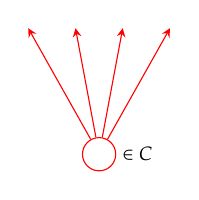
\begin{tikzpicture}
\node [rcol,vertex,large] (s) at (0, -8) {};
\coordinate (t1) at (-9,8) {};
\coordinate (t2) at (-3,8) {};
\coordinate (t3) at (3,8) {};
\coordinate (t4) at (9,8) {};
\draw [rcol,edge] (s) -- (t1);
\draw [rcol,edge] (s) -- (t2);
\draw [rcol,edge] (s) -- (t3);
\draw [rcol,edge] (s) -- (t4);
\node [annot] at (3, -8) {\rlap{$\posof C$}};
\end{tikzpicture}

    \hspace{-.75em}
    $\underset{\varepsilon}{\transformto}$
    \begin{tikzpicture}
\coordinate (s) at (0, -9.5) {};
\coordinate (t1) at (-9,8) {};
\coordinate (t2) at (-3,8) {};
\coordinate (t3) at (3,8) {};
\coordinate (t4) at (9,8) {};
\draw [dash] (s) -- (t1);
\draw [edge] (s) -- node [label] {\scriptsize$\idsubd$} (t2);
\draw [dash] (s) -- (t3);
\draw [dash] (s) -- (t4);
\end{tikzpicture}
    \quad\qquad
    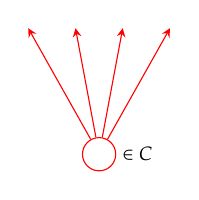
\begin{tikzpicture}
\node [rcol,vertex,large] (s) at (0, -8) {};
\coordinate (t1) at (-9,8) {};
\coordinate (t2) at (-3,8) {};
\coordinate (t3) at (3,8) {};
\coordinate (t4) at (9,8) {};
\draw [rcol,edge] (s) -- (t1);
\draw [rcol,edge] (s) -- (t2);
\draw [rcol,edge] (s) -- (t3);
\draw [rcol,edge] (s) -- (t4);
\node [annot] at (3, -8) {\rlap{$\posof C$}};
\end{tikzpicture}

    \hspace{-.75em}
    $\underset{\delta}{\transformto}$
    \hspace{.5em}
    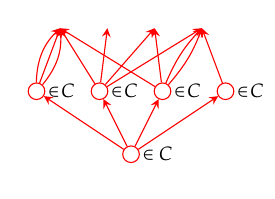
\begin{tikzpicture}
\node [rcol,vertex] (s) at (0, -8) {};
\coordinate (t1) at (-9,8) {};
\coordinate (t2) at (-3,8) {};
\coordinate (t3) at (3,8) {};
\coordinate (t4) at (9,8) {};
\node [rcol,vertex] (m1) at (-12,0) {};
\node [rcol,vertex] (m2) at (-4,0) {};
\node [rcol,vertex] (m3) at (4,0) {};
\node [rcol,vertex] (m4) at (12,0) {};
\draw [rcol,edge] (s) -- (m1);
\draw [rcol,edge] (s) -- (m2);
\draw [rcol,edge] (s) -- (m3);
\draw [rcol,edge] (s) -- (m4);

\draw [rcol,edge] (m1) -- (t1);
\draw [rcol,edge,bend left=22] (m1) to (t1);
\draw [rcol,edge,bend right=22] (m1) to (t1);

\draw [rcol,edge] (m2) -- (t1);
\draw [rcol,edge] (m2) -- (t2);
\draw [rcol,edge] (m2) -- (t3);
\draw [rcol,edge] (m2) -- (t4);

\draw [rcol,edge] (m3) -- (t1);
\draw [rcol,edge] (m3) -- (t3);
\draw [rcol,edge,bend left=10] (m3) to (t4);
\draw [rcol,edge,bend right=10] (m3) to (t4);

\draw [rcol,edge] (m4) -- (t4);

\node [annot] at (1.5, -8) {\rlap{$\posof C$}};

\node [annot] at (-10.5, 0) {\rlap{$\posof\!C$}};
\node [annot] at (-2.5, 0) {\rlap{$\posof\!C$}};
\node [annot] at (5.5, 0) {\rlap{$\posof\!C$}};
\node [annot] at (13.5, 0) {\rlap{$\posof\!C$}};
\end{tikzpicture}

  \end{center}

  \begin{center}
    \begin{tikzpicture}
\coordinate (s) at (0, -8) {};
\coordinate (t1) at (-9,8) {};
\coordinate (t2) at (-3,8) {};
\coordinate (t3) at (3,8) {};
\coordinate (t4) at (9,8) {};
\node [rcol,vertex,transparent] (m1) at (-12,0) {};
\node [rcol,vertex] (m2) at (-4,0) {};
\node [rcol,vertex,transparent] (m3) at (4,0) {};
\node [rcol,vertex,transparent] (m4) at (12,0) {};
\draw [dash] (s) -- (m1);
\draw [edge] (s) -- (m2);
\draw [dash] (s) -- (m3);
\draw [dash] (s) -- (m4);

\draw [rcol,edge,transparent] (m1) -- (t1);
\draw [rcol,edge,bend left=22,transparent] (m1) to (t1);
\draw [rcol,edge,bend right=22,transparent] (m1) to (t1);

\draw [rcol,edge] (m2) -- (t1);
\draw [rcol,edge] (m2) -- (t2);
\draw [rcol,edge] (m2) -- (t3);
\draw [rcol,edge] (m2) -- (t4);

\draw [rcol,edge,transparent] (m3) -- (t1);
\draw [rcol,edge,transparent] (m3) -- (t3);
\draw [rcol,edge,bend left=10,transparent] (m3) to (t4);
\draw [rcol,edge,bend right=10,transparent] (m3) to (t4);

\draw [rcol,edge,transparent] (m4) -- (t4);

\node at (0, -13) {$\delta \fatsemi (\varepsilon \sub \id_C)$};
\end{tikzpicture}

    \quad
    $\canoniso$
    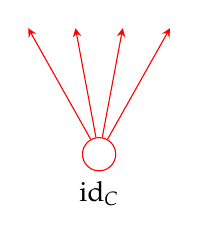
\begin{tikzpicture}
\node [rcol,vertex,large] (s) at (0, -8) {};
\coordinate (t1) at (-9,8) {};
\coordinate (t2) at (-3,8) {};
\coordinate (t3) at (3,8) {};
\coordinate (t4) at (9,8) {};
\draw [rcol,edge] (s) -- (t1);
\draw [rcol,edge] (s) -- (t2);
\draw [rcol,edge] (s) -- (t3);
\draw [rcol,edge] (s) -- (t4);

\node at (0, -13) {$\id_C$};
\end{tikzpicture}

    $\canoniso$
    \quad
    \begin{tikzpicture}
\node [rcol,vertex] (s) at (0, -8) {};
\coordinate (t1) at (-9,8) {};
\coordinate (t2) at (-3,8) {};
\coordinate (t3) at (3,8) {};
\coordinate (t4) at (9,8) {};
\coordinate (m1) at (-12,0) {};
\coordinate (m2) at (-4,0) {};
\coordinate (m3) at (4,0) {};
\coordinate (m4) at (12,0) {};
\draw [rcol,edge] (s) -- (m1);
\draw [rcol,edge] (s) -- (m2);
\draw [rcol,edge] (s) -- (m3);
\draw [rcol,edge] (s) -- (m4);

\draw [edge] (m1) -- (t1);
\draw [dash,bend left=22] (m1) to (t1);
\draw [dash,bend right=22] (m1) to (t1);

\draw [dash] (m2) -- (t1);
\draw [edge] (m2) -- (t2);
\draw [dash] (m2) -- (t3);
\draw [dash] (m2) -- (t4);

\draw [dash] (m3) -- (t1);
\draw [edge] (m3) -- (t3);
\draw [dash,bend left=10] (m3) to (t4);
\draw [dash,bend right=10] (m3) to (t4);

\draw [edge] (m4) -- (t4);

\node at (0, -13) {$\delta \fatsemi (\id_C \sub \varepsilon)$};
\end{tikzpicture}

  \end{center}

  \begin{center}
    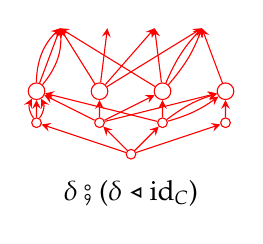
\begin{tikzpicture}
\node [rcol,vertex,small] (s) at (0, -8) {};
\coordinate (t1) at (-9,8) {};
\coordinate (t2) at (-3,8) {};
\coordinate (t3) at (3,8) {};
\coordinate (t4) at (9,8) {};

\node [rcol,vertex,small] (m1_) at (-12,-4) {};
\node [rcol,vertex,small] (m2_) at (-4,-4) {};
\node [rcol,vertex,small] (m3_) at (4,-4) {};
\node [rcol,vertex,small] (m4_) at (12,-4) {};
\draw [rcol,edge] (s) -- (m1_);
\draw [rcol,edge] (s) -- (m2_);
\draw [rcol,edge] (s) -- (m3_);
\draw [rcol,edge] (s) -- (m4_);

\node [rcol,vertex] (m1) at (-12,0) {};
\node [rcol,vertex] (m2) at (-4,0) {};
\node [rcol,vertex] (m3) at (4,0) {};
\node [rcol,vertex] (m4) at (12,0) {};

\draw [rcol,edge] (m1_) -- (m1);
\draw [rcol,edge,bend left=32] (m1_) to (m1);
\draw [rcol,edge,bend right=32] (m1_) to (m1);

\draw [rcol,edge] (m2_) -- (m1);
\draw [rcol,edge] (m2_) -- (m2);
\draw [rcol,edge] (m2_) -- (m3);
\draw [rcol,edge] (m2_) -- (m4);

\draw [rcol,edge] (m3_) -- (m1);
\draw [rcol,edge] (m3_) -- (m3);
\draw [rcol,edge,bend left=10] (m3_) to (m4);
\draw [rcol,edge,bend right=10] (m3_) to (m4);

\draw [rcol,edge] (m4_) -- (m4);


\draw [rcol,edge] (m1) -- (t1);
\draw [rcol,edge,bend left=22] (m1) to (t1);
\draw [rcol,edge,bend right=22] (m1) to (t1);

\draw [rcol,edge] (m2) -- (t1);
\draw [rcol,edge] (m2) -- (t2);
\draw [rcol,edge] (m2) -- (t3);
\draw [rcol,edge] (m2) -- (t4);

\draw [rcol,edge] (m3) -- (t1);
\draw [rcol,edge] (m3) -- (t3);
\draw [rcol,edge,bend left=10] (m3) to (t4);
\draw [rcol,edge,bend right=10] (m3) to (t4);

\draw [rcol,edge] (m4) -- (t4);

\node at (0, -13) {$\delta \fatsemi (\delta \sub \id_C)$};
\end{tikzpicture}
    \quad
    $\canoniso$
    \quad
    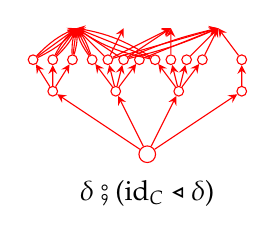
\begin{tikzpicture}
\node [rcol,vertex] (s) at (0, -8) {};
\coordinate (t1) at (-9,8) {};
\coordinate (t2) at (-3,8) {};
\coordinate (t3) at (3,8) {};
\coordinate (t4) at (9,8) {};

\node [rcol,vertex,small] (m1) at (-12,0) {};
\node [rcol,vertex,small] (m2) at (-4,0) {};
\node [rcol,vertex,small] (m3) at (4,0) {};
\node [rcol,vertex,small] (m4) at (12,0) {};
\draw [rcol,edge] (s) -- (m1);
\draw [rcol,edge] (s) -- (m2);
\draw [rcol,edge] (s) -- (m3);
\draw [rcol,edge] (s) -- (m4);

\node [rcol,vertex,small] (m11) at (-14.5,4) {};
\node [rcol,vertex,small] (m12) at (-12,4) {};
\node [rcol,vertex,small] (m13) at (-9.5,4) {};
\node [rcol,vertex,small] (m21) at (-7,4) {};
\node [rcol,vertex,small] (m22) at (-5,4) {};
\node [rcol,vertex,small] (m23) at (-3,4) {};
\node [rcol,vertex,small] (m24) at (-1,4) {};
\node [rcol,vertex,small] (m31) at (1,4) {};
\node [rcol,vertex,small] (m32) at (3,4) {};
\node [rcol,vertex,small] (m33) at (5,4) {};
\node [rcol,vertex,small] (m34) at (7,4) {};
\node [rcol,vertex,small] (m41) at (12,4) {};

\draw [rcol,edge] (m1) -- (m11);
\draw [rcol,edge] (m1) -- (m12);
\draw [rcol,edge] (m1) -- (m13);
\draw [rcol,edge] (m2) -- (m21);
\draw [rcol,edge] (m2) -- (m22);
\draw [rcol,edge] (m2) -- (m23);
\draw [rcol,edge] (m2) -- (m24);
\draw [rcol,edge] (m3) -- (m31);
\draw [rcol,edge] (m3) -- (m32);
\draw [rcol,edge] (m3) -- (m33);
\draw [rcol,edge] (m3) -- (m34);
\draw [rcol,edge] (m4) -- (m41);


\draw [rcol,edge] (m11) -- (t1);
\draw [rcol,edge,bend left=11] (m11) to (t1);
\draw [rcol,edge,bend right=11] (m11) to (t1);

\draw [rcol,edge] (m12) -- (t1);
\draw [rcol,edge,bend left=11] (m12) to (t1);
\draw [rcol,edge,bend right=11] (m12) to (t1);

\draw [rcol,edge] (m13) -- (t1);
\draw [rcol,edge,bend left=11] (m13) to (t1);
\draw [rcol,edge,bend right=11] (m13) to (t1);


\draw [rcol,edge] (m21) -- (t1);
\draw [rcol,edge,bend left=11] (m21) to (t1);
\draw [rcol,edge,bend right=11] (m21) to (t1);

\draw [rcol,edge] (m22) -- (t1);
\draw [rcol,edge] (m22) -- (t2);
\draw [rcol,edge] (m22) -- (t3);
\draw [rcol,edge] (m22) -- (t4);

\draw [rcol,edge] (m23) -- (t1);
\draw [rcol,edge] (m23) -- (t3);
\draw [rcol,edge,bend left=5] (m23) to (t4);
\draw [rcol,edge,bend right=5] (m23) to (t4);

\draw [rcol,edge] (m24) -- (t4);


\draw [rcol,edge] (m31) -- (t1);
\draw [rcol,edge,bend left=11] (m31) to (t1);
\draw [rcol,edge,bend right=11] (m31) to (t1);

\draw [rcol,edge] (m32) -- (t3);

\draw [rcol,edge] (m33) -- (t4);

\draw [rcol,edge] (m34) -- (t4);


\draw [rcol,edge] (m41) -- (t4);

\node at (0, -13) {$\delta \fatsemi (\id_C \sub \delta)$};
\end{tikzpicture}

  \end{center}

  Observe first that the right identity law forces $\posmapof{\delta}{a}_\base = a$
  for all $a \in \pos{C}$.
  Therefore the expression $\posmapof{\delta}{a}_f$ for $f \in \dir{C}{a}$ has a
  well-defined meaning.

  We gather the data for a category $\cat{C}$.
  \begin{itemize}
  \item The set of objects $\Ob(\cat{C})$ is $\pos{C}$, the set
    of positions in $C$.
  \item The set of arrows $\Arr(\cat{C})$ is
    $\sum_{a \in \pos{C}}\dir{C}{a}$, the set of all directions in $C$.
  \item The source map $s$ sends each $f \in \dir{C}{a}$ to $a$. (Hence the
    polynomial $C$ is described by the bundle
    $\Arr(\cat{C}) \bundle{s} \Ob(\cat{C})$.)
  \item The target map $t$ sends each $f \in \dir{C}{a}$ to $\posmapof{\delta}{a}_f$.
  \item The identity map $e$ sends each $a \in \pos{C}$ to
    $\dirmapof{\varepsilon}{a}{\idsubd}$.
  \item The composition map $m$ sends each pair of compatible
    arrows ${f \in \dir{C}{a}}, {g \in \dir{C}{t(f)}}$ to $\dirmapof{\delta}{a}{f \subd g}$.
  \end{itemize}

  Next, observe that if we have such prerequisite data (not laws) for
  a category, subject to just the law $s(e(a)) = a$, then we find that
  further imposing the left identity law $m(e(s(f)), f) = f$
  (and requiring that both sides are defined whenever one is)
  automatically forces the law $t(e(a)) = a$ to hold.\footnote{We have
    $m(e(s(e(a))), e(a)) = e(a)$, since the right side is defined. The
    left side reduces to $m(e(a), e(a))$. This expression only makes
    sense if $t(e(a)) = s(e(a))$, which is $a$.}  Similarly, if we
  have the law $s(m(f,g))=s(f)$ as well as $t(e(a)) = a$, then the
  associativity law $m(m(f,g),h) = m(f,m(g,h))$ forces
  $t(m(f,g)) = t(g)$.\footnote{Given that $f$ and $g$ are composable,
    we have $m(m(f,g),e(t(g))) = m(f,m(g,e(t(g))))$, since the right
    side is defined. The left side only makes sense if
    $t(f,g) = s(e(t(g)))$, which is $t(g)$.}

  We verify the data from above satisfy the laws of a category.
  \begin{itemize}
  \item The law $s(e(a)) = a$ is true by construction; $e(a)$ is a
    direction from the position $a$.
  \item The law $s(m(f, g)) = s(f)$ is true by construction; $m(f, g)$
    is a direction from the position $s(f)$.
  \item The left identity law $m(e(s(f)), f) = f$ is directly
    expressed by the comonoid left identity law, which identifies
    ${\anydirmapof{\delta}{\anydirmapof{\varepsilon}{\idsubd} \subd f}}$
    with $f$ whenever this makes sense.\iffalse\footnote{Meaning,
        there are $u$ and $v$ such that
        ${\dirmapof{\delta}{u}{\dirmapof{\varepsilon}{v}{\idsubd} \subd
            f}}$ specifies a direction from position $a$ $\iff$ $f$
        specifies a direction from position $a$; in this case, the
        former and latter are equal.}\fi
  \item The right identity law $m(f, e(t(f))) = f$ is directly
    expressed by the comonoid right identity law, which identifies
    ${\anydirmapof{\delta}{f \subd \anydirmapof{\varepsilon}{\idsubd}}}$
    with $f$ whenever this makes sense.
  \item The associativity law $m(m(f, g), h) = m(f, m(g, h))$ is
    directly expressed by the comonoid associativity law, which
    identifies
    ${\anydirmapof{\delta}{\anydirmapof{\delta}{f \subd g} \subd h}}$ with
    ${\anydirmapof{\delta}{f \subd \anydirmapof{\delta}{g \subd h}}}$ whenever this makes sense.
  \item The law $t(e(a)) = a$ is forced to hold (due to the comonoid
    left identity law).
  \item The law $t(m(f, g)) = t(g)$ is forced to hold (due to the
    comonoid associativity law).
  \end{itemize}

  Conversely, let $\cat{C}$ be a category. We immediately obtain the
  bundle ${\Arr(\cat{C})\bundle{s}\Ob(\cat{C})}$. Let $C$ denote
  the polynomial described by this bundle (the ``outfacing polynomial''
  of $\cat{C}$). We will exhibit a comonoid struture on $C$.
  \begin{itemize}
  \item The counit $\varepsilon$ singles out the identity in each
    object's set of outfacing maps.
  \item The comultiplication $\delta$ endows each object $a$ with the
    map $\dirmap{\delta}{a}$ sending $f \subd g$ to $m(f, g)$ for all
    arrows of the form $f: a \to b$, $g: b \to c$ (through which the
    map $\posmap{\delta}$ is implicit).
  \end{itemize}

  The above processes of translation between the prerequisite data
  (not laws) for a category subject to just $s(e(a)) = a$ and
  $s(m(f, g)) = g$, and the prerequisite data (not laws) for a
  polynomial comonoid subject to just
  $\posmapof{\delta}{a}_\base = a$, are inverse by
  construction. Moreover, we saw earlier that the identity and
  associativity comonoid laws, in this context, directly translate
  to the identity and associativity category laws.
\end{proof}

\begin{prop}
  A polynomial right comodule amounts to a family of copresheaves.
\end{prop}
\begin{proof}
  Let $D$ be a polynomial comonoid with counit $\varepsilon$ and
  comultiplication $\delta$, and let $M$ be a right comodule on
  $D$. Denote right comodule comultiplication by $\rho$.

  \begin{center}
    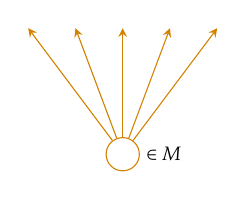
\begin{tikzpicture}
\node [ycol,vertex,large] (s) at (0, -8) {};
\coordinate (t1) at (-12,8) {};
\coordinate (t2) at (-6,8) {};
\coordinate (t3) at (0,8) {};
\coordinate (t4) at (6,8) {};
\coordinate (t5) at (12,8) {};
\draw [ycol,edge] (s) -- (t1);
\draw [ycol,edge] (s) -- (t2);
\draw [ycol,edge] (s) -- (t3);
\draw [ycol,edge] (s) -- (t4);
\draw [ycol,edge] (s) -- (t5);
\node [annot] at (3, -8) {\rlap{$\posof M$}};
\end{tikzpicture}

    \hspace{-.75em}
    $\underset{\rho}{\transformto}$
    \hspace{.5em}
    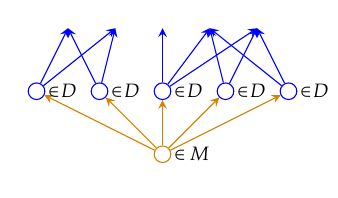
\begin{tikzpicture}
\node [ycol,vertex] (s) at (0, -8) {};
\coordinate (t1) at (-12,8) {};
\coordinate (t2) at (-6,8) {};
\coordinate (t3) at (-0,8) {};
\coordinate (t4) at (6,8) {};
\coordinate (t5) at (12,8) {};
\node [bcol,vertex] (m1) at (-16,0) {};
\node [bcol,vertex] (m2) at (-8,0) {};
\node [bcol,vertex] (m3) at (0,0) {};
\node [bcol,vertex] (m4) at (8,0) {};
\node [bcol,vertex] (m5) at (16,0) {};
\draw [ycol,edge] (s) -- (m1);
\draw [ycol,edge] (s) -- (m2);
\draw [ycol,edge] (s) -- (m3);
\draw [ycol,edge] (s) -- (m4);
\draw [ycol,edge] (s) -- (m5);

\draw [bcol,edge] (m1) -- (t1);
\draw [bcol,edge] (m1) -- (t2);

\draw [bcol,edge] (m2) -- (t1);
\draw [bcol,edge] (m2) -- (t2);

\draw [bcol,edge] (m3) -- (t3);
\draw [bcol,edge] (m3) -- (t4);
\draw [bcol,edge] (m3) -- (t5);

\draw [bcol,edge] (m4) -- (t4);
\draw [bcol,edge] (m4) -- (t5);

\draw [bcol,edge] (m5) -- (t4);
\draw [bcol,edge] (m5) -- (t5);

\node [annot] at (1.5, -8) {\rlap{$\posof M$}};

\node [annot] at (-14.5, 0) {\rlap{$\posof\!D$}};
\node [annot] at (-6.5, 0) {\rlap{$\posof\!D$}};
\node [annot] at (1.5, 0) {\rlap{$\posof\!D$}};
\node [annot] at (9.5, 0) {\rlap{$\posof\!D$}};
\node [annot] at (17.5, 0) {\rlap{$\posof\!D$}};
\end{tikzpicture}

  \end{center}

  \begin{center}
    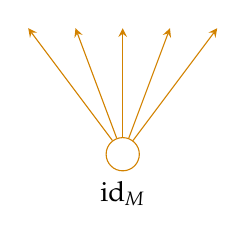
\begin{tikzpicture}
\node [ycol,vertex,large] (s) at (0, -8) {};
\coordinate (t1) at (-12,8) {};
\coordinate (t2) at (-6,8) {};
\coordinate (t3) at (0,8) {};
\coordinate (t4) at (6,8) {};
\coordinate (t5) at (12,8) {};
\draw [ycol,edge] (s) -- (t1);
\draw [ycol,edge] (s) -- (t2);
\draw [ycol,edge] (s) -- (t3);
\draw [ycol,edge] (s) -- (t4);
\draw [ycol,edge] (s) -- (t5);

\node at (0, -13) {$\id_M$};
\end{tikzpicture}

    $\canoniso$
    \quad
    \begin{tikzpicture}
\node [ycol,vertex] (s) at (0, -8) {};
\coordinate (t1) at (-12,8) {};
\coordinate (t2) at (-6,8) {};
\coordinate (t3) at (0,8) {};
\coordinate (t4) at (6,8) {};
\coordinate (t5) at (12,8) {};

\coordinate (m1) at (-16,0) {};
\coordinate (m2) at (-8,0) {};
\coordinate (m3) at (0,0) {};
\coordinate (m4) at (8,0) {};
\coordinate (m5) at (16,0) {};

\draw [ycol,edge] (s) -- (m1);
\draw [ycol,edge] (s) -- (m2);
\draw [ycol,edge] (s) -- (m3);
\draw [ycol,edge] (s) -- (m4);
\draw [ycol,edge] (s) -- (m5);

\draw [edge] (m1) -- (t1);
\draw [dash] (m1) -- (t2);

\draw [dash] (m2) -- (t1);
\draw [edge] (m2) -- (t2);

\draw [edge] (m3) -- (t3);
\draw [dash] (m3) -- (t4);
\draw [dash] (m3) -- (t5);

\draw [edge] (m4) -- (t4);
\draw [dash] (m4) -- (t5);

\draw [dash] (m5) -- (t4);
\draw [edge] (m5) -- (t5);

\node at (0, -13) {$\rho \fatsemi (\id_M \sub \varepsilon)$};
\end{tikzpicture}

  \end{center}

  \begin{center}
    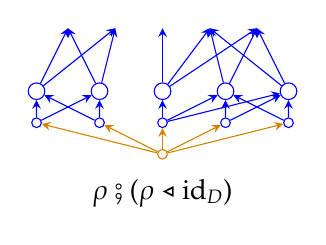
\begin{tikzpicture}
\node [ycol,vertex,small] (s) at (0, -8) {};
\coordinate (t1) at (-12,8) {};
\coordinate (t2) at (-6,8) {};
\coordinate (t3) at (-0,8) {};
\coordinate (t4) at (6,8) {};
\coordinate (t5) at (12,8) {};

\node [bcol,vertex,small] (m1) at (-16,-4) {};
\node [bcol,vertex,small] (m2) at (-8,-4) {};
\node [bcol,vertex,small] (m3) at (0,-4) {};
\node [bcol,vertex,small] (m4) at (8,-4) {};
\node [bcol,vertex,small] (m5) at (16,-4) {};

\node [bcol,vertex] (m1_) at (-16,0) {};
\node [bcol,vertex] (m2_) at (-8,0) {};
\node [bcol,vertex] (m3_) at (0,0) {};
\node [bcol,vertex] (m4_) at (8,0) {};
\node [bcol,vertex] (m5_) at (16,0) {};

\draw [ycol,edge] (s) -- (m1);
\draw [ycol,edge] (s) -- (m2);
\draw [ycol,edge] (s) -- (m3);
\draw [ycol,edge] (s) -- (m4);
\draw [ycol,edge] (s) -- (m5);

\draw [bcol,edge] (m1) -- (m1_);
\draw [bcol,edge] (m1) -- (m2_);

\draw [bcol,edge] (m2) -- (m1_);
\draw [bcol,edge] (m2) -- (m2_);

\draw [bcol,edge] (m3) -- (m3_);
\draw [bcol,edge] (m3) -- (m4_);
\draw [bcol,edge] (m3) -- (m5_);

\draw [bcol,edge] (m4) -- (m4_);
\draw [bcol,edge] (m4) -- (m5_);

\draw [bcol,edge] (m5) -- (m4_);
\draw [bcol,edge] (m5) -- (m5_);

\draw [bcol,edge] (m1_) -- (t1);
\draw [bcol,edge] (m1_) -- (t2);

\draw [bcol,edge] (m2_) -- (t1);
\draw [bcol,edge] (m2_) -- (t2);

\draw [bcol,edge] (m3_) -- (t3);
\draw [bcol,edge] (m3_) -- (t4);
\draw [bcol,edge] (m3_) -- (t5);

\draw [bcol,edge] (m4_) -- (t4);
\draw [bcol,edge] (m4_) -- (t5);

\draw [bcol,edge] (m5_) -- (t4);
\draw [bcol,edge] (m5_) -- (t5);


\node at (0, -13) {$\rho \fatsemi (\rho \sub \id_D)$};
\end{tikzpicture}

    \quad
    $\canoniso$
    \quad
    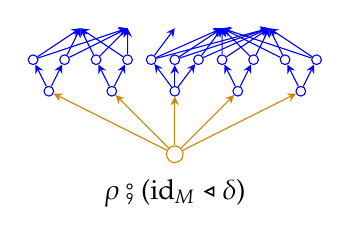
\begin{tikzpicture}
\node [ycol,vertex] (s) at (0, -8) {};
\coordinate (t1) at (-12,8) {};
\coordinate (t2) at (-6,8) {};
\coordinate (t3) at (-0,8) {};
\coordinate (t4) at (6,8) {};
\coordinate (t5) at (12,8) {};

\node [bcol,vertex,small] (m1) at (-16,0) {};
\node [bcol,vertex,small] (m2) at (-8,0) {};
\node [bcol,vertex,small] (m3) at (0,0) {};
\node [bcol,vertex,small] (m4) at (8,0) {};
\node [bcol,vertex,small] (m5) at (16,0) {};

\node [bcol,vertex,small] (m11) at (-18,4) {};
\node [bcol,vertex,small] (m12) at (-14,4) {};
\node [bcol,vertex,small] (m21) at (-10,4) {};
\node [bcol,vertex,small] (m22) at (-6,4) {};
\node [bcol,vertex,small] (m31) at (-3,4) {};
\node [bcol,vertex,small] (m32) at (0,4) {};
\node [bcol,vertex,small] (m33) at (3,4) {};
\node [bcol,vertex,small] (m41) at (6,4) {};
\node [bcol,vertex,small] (m42) at (10,4) {};
\node [bcol,vertex,small] (m51) at (14,4) {};
\node [bcol,vertex,small] (m52) at (18,4) {};

\draw [ycol,edge] (s) -- (m1);
\draw [ycol,edge] (s) -- (m2);
\draw [ycol,edge] (s) -- (m3);
\draw [ycol,edge] (s) -- (m4);
\draw [ycol,edge] (s) -- (m5);


\draw [bcol,edge] (m1) -- (m11);
\draw [bcol,edge] (m1) -- (m12);

\draw [bcol,edge] (m2) -- (m21);
\draw [bcol,edge] (m2) -- (m22);

\draw [bcol,edge] (m3) -- (m31);
\draw [bcol,edge] (m3) -- (m32);
\draw [bcol,edge] (m3) -- (m33);

\draw [bcol,edge] (m4) -- (m41);
\draw [bcol,edge] (m4) -- (m42);

\draw [bcol,edge] (m5) -- (m51);
\draw [bcol,edge] (m5) -- (m52);


\draw [bcol,edge] (m11) -- (t1);
\draw [bcol,edge] (m11) -- (t2);

\draw [bcol,edge] (m12) -- (t1);
\draw [bcol,edge] (m12) -- (t2);

\draw [bcol,edge] (m21) -- (t1);
\draw [bcol,edge] (m21) -- (t2);

\draw [bcol,edge] (m22) -- (t1);
\draw [bcol,edge] (m22) -- (t2);

\draw [bcol,edge] (m31) -- (t3);
\draw [bcol,edge] (m31) -- (t4);
\draw [bcol,edge] (m31) -- (t5);

\draw [bcol,edge] (m32) -- (t4);
\draw [bcol,edge] (m32) -- (t5);

\draw [bcol,edge] (m33) -- (t4);
\draw [bcol,edge] (m33) -- (t5);

\draw [bcol,edge] (m41) -- (t4);
\draw [bcol,edge] (m41) -- (t5);

\draw [bcol,edge] (m42) -- (t4);
\draw [bcol,edge] (m42) -- (t5);

\draw [bcol,edge] (m51) -- (t4);
\draw [bcol,edge] (m51) -- (t5);

\draw [bcol,edge] (m52) -- (t4);
\draw [bcol,edge] (m52) -- (t5);


\node at (0, -13) {$\rho \fatsemi (\id_M \sub \delta)$};
\end{tikzpicture}

  \end{center}

  Observe first that the identity law forces $\posmapof{\rho}{a}_\base = a$
  for all $a \in \pos{M}$.
  Therefore the expression $\posmapof{\rho}{a}_z$ for $z \in \dir{M}{a}$ has a
  well-defined meaning.

  Let $\cat{D}$ be the category corresponding to $D$. We gather the
  data for a family of copresheaves $\{Z_a\}_{a \in A}$ on $\cat{D}$.
  \begin{itemize}
  \item The family's indexing set $A$ is $\pos{M}$, the set
    of positions in $M$.
  \item The total set of elements $\sum_{d \in \Ob(\cat{D})}Z_a(d)$ in
    $Z_a$ is $\dir{M}{a}$, the set of directions from $a$.
  \item The bundle map $t$ assigning each element $z$ in $Z_a$ its indexing
    object in $\Ob(\cat{D}) = \pos{D}$ is given by $\posmapof{\rho}{a}_z$.
  \item The multiplication map $m$ sends each element $z \in Z_a(d)$ and compatible
    arrow $f \in \dir{D}{d}$ to $\dirmapof{\rho}{a}{z \subd f}$.
  \end{itemize}
  
  Next, observe that if we have such prerequisite data (not laws) for
  a copresheaf on $\cat{D}$, then we find that imposing the copresheaf
  associativity law $m(m(z, f), g) = m(z, m(f, g))$ forces the law
  $t(m(z,f)) = t(f)$ to hold.\footnote{Given that $z$ and $f$ are
    composable, we have $m(m(z,f),e(t(f))) = m(z,m(f,e(t(f))))$, since
    the right side is defined. The left side only makes sense if
    $t(z,f) = s(e(t(f)))$, which is $t(f)$.} (The argument works the same
  for copresheaves as it does for categories.)

  We verify each $Z_a$ satisfies the laws of a copresheaf on $\cat{D}$.
  \begin{itemize}
  \item The identity law $m(z, e(t(z))) = z$ is directly expressed by
    the right comodule identity law, which identifies
    ${\anydirmapof{\rho}{z \subd \anydirmapof{\varepsilon}{\idsubd}}}$
    whenever this makes sense.
  \item The associativity law $m(m(z, f), g) = m(z, m(f, g))$ is
    directly expressed by the right comodule associativity law, which
    identifies
    ${\anydirmapof{\rho}{\anydirmapof{\rho}{z \subd f} \subd g}}$ with
    ${\anydirmapof{\rho}{z \subd \anydirmapof{\delta}{f \subd g}}}$ whenever this makes sense.
  \item The law $t(m(z, f)) = t(f)$ is forced to hold (due to the
    right comodule associativity law).
  \end{itemize}

  Conversely, let $\{Z_a\}_{a \in A}$ be a family of copresheaves on
  $\cat{D}$. Let $M$ denote the polynomial described by the family of
  total sets of elements
  $\{\sum_{d \in \Ob(\cat{D})}Z_a(d)\}_{a \in A}$. We will exhibit a right
  $D$-comodule struture on $M$.
  \begin{itemize}
  \item The right comodule comultiplication $\rho$ endows each position $a \in A$ with
    the map $\dirmap{\rho}{a}$ sending each $z \subd f$ to $m(z, f)$ for
    all $z \in Z_a(d), f: d \to d' \in \cat{D}$. This implicitly
    determines $\posmapof{\rho}{a}$ as long as the domain of $\dirmap{\rho}{a}$ is
    nonempty; otherwise let $\posmapof{\rho}{a}$ be the unique position in
    $M \sub D$ with $\posmapof{\rho}{a}_\base = a$.
  \end{itemize}

  The above processes of translation between the prerequisite data
  (not laws) for a family of presheaves on $\cat{D}$, and the
  prerequisite data (not laws) for a right $D$-comodule subject to just
  $\posmapof{\rho}{a}_\base = a$, are inverse by
  construction. Moreover, we saw earlier that the identity and
  associativity right comodule laws, in this context, directly translate
  to the identity and associativity copresheaf laws.
\end{proof}

\begin{prop}
  A polynomial left comodule amounts to a copresheaf and a presheaf on that
  copresheaf's category of elements.
\end{prop}
\begin{proof}
  Let $C$ be a polynomial comonoid with counit $\varepsilon$ and
  comultiplication $\delta$, and let $M$ be a left comodule on
  $C$. Denote left comodule comultiplication by $\lambda$.

  \begin{center}
    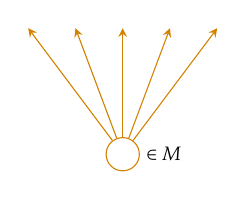
\begin{tikzpicture}
\node [ycol,vertex,large] (s) at (0, -8) {};
\coordinate (t1) at (-12,8) {};
\coordinate (t2) at (-6,8) {};
\coordinate (t3) at (0,8) {};
\coordinate (t4) at (6,8) {};
\coordinate (t5) at (12,8) {};
\draw [ycol,edge] (s) -- (t1);
\draw [ycol,edge] (s) -- (t2);
\draw [ycol,edge] (s) -- (t3);
\draw [ycol,edge] (s) -- (t4);
\draw [ycol,edge] (s) -- (t5);
\node [annot] at (3, -8) {\rlap{$\posof M$}};
\end{tikzpicture}

    \hspace{-.75em}
    $\underset{\lambda}{\transformto}$
    \hspace{.5em}
    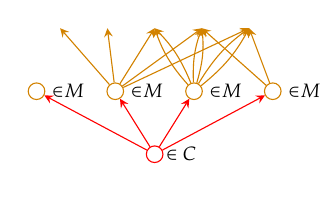
\begin{tikzpicture}
\node [rcol,vertex] (s) at (0, -8) {};
\coordinate (t1) at (-12,8) {};
\coordinate (t2) at (-6,8) {};
\coordinate (t3) at (0,8) {};
\coordinate (t4) at (6,8) {};
\coordinate (t5) at (12,8) {};
\node [ycol,vertex] (m1) at (-15,0) {};
\node [ycol,vertex] (m2) at (-5,0) {};
\node [ycol,vertex] (m3) at (5,0) {};
\node [ycol,vertex] (m4) at (15,0) {};
\draw [rcol,edge] (s) -- (m1);
\draw [rcol,edge] (s) -- (m2);
\draw [rcol,edge] (s) -- (m3);
\draw [rcol,edge] (s) -- (m4);

\draw [ycol,edge] (m2) -- (t1);
\draw [ycol,edge] (m2) -- (t2);
\draw [ycol,edge] (m2) -- (t3);
\draw [ycol,edge] (m2) -- (t4);
\draw [ycol,edge] (m2) -- (t5);

\draw [ycol,edge,bend left=11] (m3) to (t3);
\draw [ycol,edge,bend right=11] (m3) to (t3);
\draw [ycol,edge,bend left=11] (m3) to (t4);
\draw [ycol,edge,bend right=11] (m3) to (t4);
\draw [ycol,edge,bend left=11] (m3) to (t5);
\draw [ycol,edge,bend right=11] (m3) to (t5);

\draw [ycol,edge] (m4) -- (t4);
\draw [ycol,edge] (m4) -- (t5);

\node [annot] at (1.5, -8) {\rlap{$\posof C$}};

\node [annot] at (-13, 0) {\rlap{$\posof\!M$}};
\node [annot] at (-3, 0) {\rlap{$\posof\!M$}};
\node [annot] at (7, 0) {\rlap{$\posof\!M$}};
\node [annot] at (17, 0) {\rlap{$\posof\!M$}};
\end{tikzpicture}

  \end{center}

  \begin{center}
    \begin{tikzpicture}
\coordinate (s) at (0, -8) {};
\coordinate (t1) at (-12,8) {};
\coordinate (t2) at (-6,8) {};
\coordinate (t3) at (0,8) {};
\coordinate (t4) at (6,8) {};
\coordinate (t5) at (12,8) {};

\node [ycol,vertex,transparent] (m1) at (-15,0) {};
\node [ycol,vertex] (m2) at (-5,0) {};
\node [ycol,vertex,transparent] (m3) at (5,0) {};
\node [ycol,vertex,transparent] (m4) at (15,0) {};
\draw [dash] (s) -- (m1);
\draw [edge] (s) -- (m2);
\draw [dash] (s) -- (m3);
\draw [dash] (s) -- (m4);

\draw [ycol,edge] (m2) -- (t1);
\draw [ycol,edge] (m2) -- (t2);
\draw [ycol,edge] (m2) -- (t3);
\draw [ycol,edge] (m2) -- (t4);
\draw [ycol,edge] (m2) -- (t5);

\draw [ycol,edge,transparent,bend left=11] (m3) to (t3);
\draw [ycol,edge,transparent,bend right=11] (m3) to (t3);
\draw [ycol,edge,transparent,bend left=11] (m3) to (t4);
\draw [ycol,edge,transparent,bend right=11] (m3) to (t4);
\draw [ycol,edge,transparent,bend left=11] (m3) to (t5);
\draw [ycol,edge,transparent,bend right=11] (m3) to (t5);

\draw [ycol,transparent,edge] (m4) -- (t4);
\draw [ycol,transparent,edge] (m4) -- (t5);

\node at (0, -13) {$\lambda \fatsemi (\varepsilon \sub \id_M)$};
\end{tikzpicture}

    \quad
    $\canoniso$
    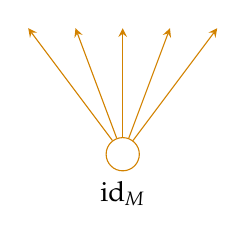
\begin{tikzpicture}
\node [ycol,vertex,large] (s) at (0, -8) {};
\coordinate (t1) at (-12,8) {};
\coordinate (t2) at (-6,8) {};
\coordinate (t3) at (0,8) {};
\coordinate (t4) at (6,8) {};
\coordinate (t5) at (12,8) {};
\draw [ycol,edge] (s) -- (t1);
\draw [ycol,edge] (s) -- (t2);
\draw [ycol,edge] (s) -- (t3);
\draw [ycol,edge] (s) -- (t4);
\draw [ycol,edge] (s) -- (t5);

\node at (0, -13) {$\id_M$};
\end{tikzpicture}

  \end{center}
  
  \begin{center}
    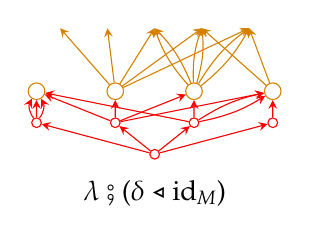
\begin{tikzpicture}
\node [rcol,vertex,small] (s) at (0, -8) {};
\coordinate (t1) at (-12,8) {};
\coordinate (t2) at (-6,8) {};
\coordinate (t3) at (0,8) {};
\coordinate (t4) at (6,8) {};
\coordinate (t5) at (12,8) {};


\node [rcol,vertex,small] (m1_) at (-15,-4) {};
\node [rcol,vertex,small] (m2_) at (-5,-4) {};
\node [rcol,vertex,small] (m3_) at (5,-4) {};
\node [rcol,vertex,small] (m4_) at (15,-4) {};

\node [ycol,vertex] (m1) at (-15,0) {};
\node [ycol,vertex] (m2) at (-5,0) {};
\node [ycol,vertex] (m3) at (5,0) {};
\node [ycol,vertex] (m4) at (15,0) {};

\draw [rcol,edge] (s) -- (m1_);
\draw [rcol,edge] (s) -- (m2_);
\draw [rcol,edge] (s) -- (m3_);
\draw [rcol,edge] (s) -- (m4_);

\draw [rcol,edge] (m1_) -- (m1);
\draw [rcol,edge,bend left=32] (m1_) to (m1);
\draw [rcol,edge,bend right=32] (m1_) to (m1);

\draw [rcol,edge] (m2_) -- (m1);
\draw [rcol,edge] (m2_) -- (m2);
\draw [rcol,edge] (m2_) -- (m3);
\draw [rcol,edge] (m2_) -- (m4);

\draw [rcol,edge] (m3_) -- (m1);
\draw [rcol,edge] (m3_) -- (m3);
\draw [rcol,edge,bend left=10] (m3_) to (m4);
\draw [rcol,edge,bend right=10] (m3_) to (m4);

\draw [rcol,edge] (m4_) -- (m4);


\draw [ycol,edge] (m2) -- (t1);
\draw [ycol,edge] (m2) -- (t2);
\draw [ycol,edge] (m2) -- (t3);
\draw [ycol,edge] (m2) -- (t4);
\draw [ycol,edge] (m2) -- (t5);

\draw [ycol,edge,bend left=11] (m3) to (t3);
\draw [ycol,edge,bend right=11] (m3) to (t3);
\draw [ycol,edge,bend left=11] (m3) to (t4);
\draw [ycol,edge,bend right=11] (m3) to (t4);
\draw [ycol,edge,bend left=11] (m3) to (t5);
\draw [ycol,edge,bend right=11] (m3) to (t5);

\draw [ycol,edge] (m4) -- (t4);
\draw [ycol,edge] (m4) -- (t5);


\node at (0, -13) {$\lambda \fatsemi (\delta \sub \id_M)$};
\end{tikzpicture}

    \quad
    $\canoniso$
    \quad
    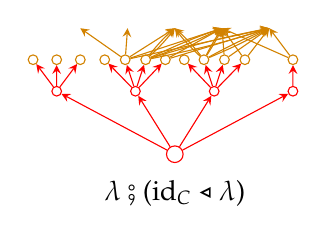
\begin{tikzpicture}
\node [rcol,vertex] (s) at (0, -8) {};
\coordinate (t1) at (-12,8) {};
\coordinate (t2) at (-6,8) {};
\coordinate (t3) at (0,8) {};
\coordinate (t4) at (6,8) {};
\coordinate (t5) at (12,8) {};

\node [ycol,vertex,small] (m11) at (-18,4) {};
\node [ycol,vertex,small] (m12) at (-15,4) {};
\node [ycol,vertex,small] (m13) at (-12,4) {};
\node [ycol,vertex,small] (m21) at (-8.9,4) {};
\node [ycol,vertex,small] (m22) at (-6.3,4) {};
\node [ycol,vertex,small] (m23) at (-3.7,4) {};
\node [ycol,vertex,small] (m24) at (-1.2,4) {};
\node [ycol,vertex,small] (m31) at (1.2,4) {};
\node [ycol,vertex,small] (m32) at (3.7,4) {};
\node [ycol,vertex,small] (m33) at (6.3,4) {};
\node [ycol,vertex,small] (m34) at (8.9,4) {};
\node [ycol,vertex,small] (m41) at (15,4) {};

\node [rcol,vertex,small] (m1) at (-15,0) {};
\node [rcol,vertex,small] (m2) at (-5,0) {};
\node [rcol,vertex,small] (m3) at (5,0) {};
\node [rcol,vertex,small] (m4) at (15,0) {};

\draw [rcol,edge] (m1) -- (m11);
\draw [rcol,edge] (m1) -- (m12);
\draw [rcol,edge] (m1) -- (m13);
\draw [rcol,edge] (m2) -- (m21);
\draw [rcol,edge] (m2) -- (m22);
\draw [rcol,edge] (m2) -- (m23);
\draw [rcol,edge] (m2) -- (m24);
\draw [rcol,edge] (m3) -- (m31);
\draw [rcol,edge] (m3) -- (m32);
\draw [rcol,edge] (m3) -- (m33);
\draw [rcol,edge] (m3) -- (m34);
\draw [rcol,edge] (m4) -- (m41);

\draw [rcol,edge] (s) -- (m1);
\draw [rcol,edge] (s) -- (m2);
\draw [rcol,edge] (s) -- (m3);
\draw [rcol,edge] (s) -- (m4);

\draw [ycol,edge] (m22) -- (t1);
\draw [ycol,edge] (m22) -- (t2);
\draw [ycol,edge] (m22) -- (t3);
\draw [ycol,edge] (m22) -- (t4);
\draw [ycol,edge] (m22) -- (t5);

\draw [ycol,edge,bend left=5] (m23) to (t3);
\draw [ycol,edge,bend right=5] (m23) to (t3);
\draw [ycol,edge,bend left=3] (m23) to (t4);
\draw [ycol,edge,bend right=3] (m23) to (t4);
\draw [ycol,edge,bend left=3] (m23) to (t5);
\draw [ycol,edge,bend right=3] (m23) to (t5);

\draw [ycol,edge] (m24) -- (t4);
\draw [ycol,edge] (m24) -- (t5);


\draw [ycol,edge,bend left=5] (m32) to (t3);
\draw [ycol,edge,bend right=5] (m32) to (t3);
\draw [ycol,edge,bend left=3] (m32) to (t4);
\draw [ycol,edge,bend right=3] (m32) to (t4);
\draw [ycol,edge,bend left=3] (m32) to (t5);
\draw [ycol,edge,bend right=3] (m32) to (t5);
\draw [ycol,edge] (m33) -- (t4);
\draw [ycol,edge] (m33) -- (t5);
\draw [ycol,edge] (m34) -- (t4);
\draw [ycol,edge] (m34) -- (t5);


\draw [ycol,edge] (m41) -- (t4);
\draw [ycol,edge] (m41) -- (t5);


\node at (0, -13) {$\lambda \fatsemi (\id_C \sub \lambda)$};
\end{tikzpicture}

  \end{center}

  Let $\cat{C}$ be the category corresponding to $C$. We gather the
  data for a copresheaf $X$ on $\cat{C}$.
  \begin{itemize}
  \item The total set of elements $\sum_{c \in \Ob(\cat{C})}X(c)$ in
    $X$ is $\pos{M}$, the set of positions in $M$.
  \item The bundle map $t$ assigning each element $x$ in $X$ its indexing
    object in $\Ob(\cat{C}) = \pos{C}$ is given by $\posmapof{\lambda}{x}_\base$.
  \item The multiplication map $m$ sends each element $x \in \pos{M}$
    and compatible arrow $f \in \dir{C}{t(x)}$ to
    $\posmapof{\lambda}{x}_f$.
  \end{itemize}

  Now we gather the remaining data of a presheaf $Z$ on
  $\int_{\cat{C}}X$, the category of elements of $X$. (We will have
  accumulated the data sans laws of a copresheaf on $\cat{C}$ and
  presheaf on its category of elements; we are still yet to
  verify $X$ satisfies the laws of a copresheaf on $\cat{C}$.)
  \begin{itemize}
  \item The set $Z(x)$ for $x \in \Ob(\int_{\cat{C}}X) = \pos{M}$ is
    $\dir{M}{x}$, the set of directions from $x$. Hence we obtain the
    bundle map $s$ from the total set of elements
    $\sum_{x \in \Ob(\int_{\cat{C}}X)}Z(x)$ to $\Ob(\int_{\cat{C}}X)$
    sending each $z \in Z(x)$ to $x$.
  \item The multiplication map $m$ sends each arrow $\atel{f}{x}: x \to w$
    (in $\int_{\cat{C}}X$, lying over $f: t(x) \to t(w)$ in $\cat{C}$)
    and $w$-indexed element $z \in Z(w) = \dir{M}{w}$ to
    $\dirmapof{\lambda}{x}{f \subd z}$.

    (To be clear, the domain of this map is the set of tuples
    $(x, f, z)$ such that $t(x) = s(f)$ and $m(x, f) = s(z)$. This is
    indeed the set of pairs $(\atel{f}{x}, z)$ that should belong in the
    domain of multiplication for our presheaf on $\int_{\cat{C}}X$,
    since an arrow $\atel{f}{x}$ in $\int_{\cat{C}}X$ is a pair $(x, f)$ such
    that $t(x) = s(f)$, and the target of this arrow is $m(x, f)$.)
  \end{itemize}

  We will also use the following notation for identities and
  composition in $\int_{\cat{C}}X$.
  \begin{itemize}
  \item If $x$ is an element of $X$, then $e(x)$ will refer to
    $\atel{e(t(x))}{x}$.
  \item If $\atel{f}{x}$ and $\atel{g}{m(x,f)}$ are composable arrows in
    $\int_{\cat{C}}X$, then $m(\atel{f}{x}, \atel{g}{m(x,f)})$ will refer to
    $\atel{m(f, g)}{x}$.
  \end{itemize}

  We verify $X$ satisfies the laws of a copresheaf on $\cat{C}$.
  \begin{itemize}
  \item The identity law $m(x, e(t(x))) = x$ is the content of the left
    comodule identity law as regards positions, which says that
    $\posmapof{\lambda}{x}_{\left(\dirmapof{\varepsilon}{\posmapof{\lambda}{x}_\base}{\idsubd}\right)} = x$.
  \item The associativity law $m(m(x, f), g) = m(x, m(f, g))$ is the
    content of the left comodule associativity law as regards positions,
    which says that
    $\posmapof{\lambda}{\posmapof{\lambda}{x}_f}_g =
    \posmapof{\lambda}{x}_{\left(\dirmapof{\delta}{\posmapof{\lambda}{x}_\base)}{f
        \subd g}\right)}$.
  \item The law $t(m(x, f)) = t(f)$ is forced to hold by the
    associativity law, as we have seen previously.
  \end{itemize}
  
  Now we verify $Z$ satisfies the laws of a presheaf on $\int_{\cat{C}}X$.
  \begin{itemize}
  \item The identity law $m(e(s(z)), z) = z$ is the content of the left
    comodule identity law as regards directions, which identifies
    ${\anydirmapof{\lambda}{\anydirmapof{\varepsilon}{\idsubd} \subd z}}$
    with $z$ whenever this makes sense.
  \item The associativity law
    $m(m(\atel{f}{x}, \atel{g}{m(x,f)}), z) = m(\atel{f}{x}, m(\atel{g}{m(x,f)}, z))$ is the
    content of the left comodule associativity law as regards
    directions, which identifies
    ${\anydirmapof{\lambda}{\anydirmapof{\delta}{f \subd g} \subd z}}$
    with
    ${\anydirmapof{\lambda}{f \subd \anydirmapof{\lambda}{g \subd z}}}$
    whenever this makes sense.
  \item The law $s(m(\atel{f}{x}, z)) = s(\atel{f}{x})$ is forced to hold by the
    associativity law, as we have seen previously (in the dual
    scenario).
  \end{itemize}

  Conversely, let $X$ be a copresheaf on $\cat{C}$ and $Z$ be a
  presheaf on $\int_{\cat{C}}X$. We immediately obtain the bundle
  ${\sum_{x \in \Ob(\int_{\cat{C}}X)}Z(x) \bundle{s}
    \Ob(\int_{\cat{C}}X)}$. Let $M$ denote the polynomial described by
  this bundle. We will exhibit a left $C$-comodule struture on $M$.
  \begin{itemize}
  \item The left comodule comultiplication $\lambda$ is defined on
    positions by $\posmapof{\lambda}{x}_\base = t(x)$ and
    $\posmapof{\lambda}{x}_f = m(x,f)$ for all ${f \in \dir{C}{t(x)}}$.
  \item For each position $x$, the map $\dirmap{\lambda}{x}$ sends each
    $f \subd z$ to $m(\atel{f}{x}, z)$ for all
    ${f \in \dir{C}{t(x)}}, {z \in Z(m(x,f))}$.
  \end{itemize}

  The above processes of translation between the prerequisite data
  (not laws) for a presheaf on the category of elements of a
  copresheaf on $\cat{C}$, and the prerequisite data (not laws) for a
  left $C$-comodule, are inverse by construction. Moreover, we saw
  earlier that the identity and associativity left comodule
  laws, in this context, directly translate to the identity and
  associativity copresheaf and presheaf laws.
\end{proof}

\begin{prop}
  Polynomial bicomodules are prafunctors between presheaf categories.
\end{prop}
\begin{proof}
  Let $C$ and $D$ be polynomial comonoids and let $M$ a bicomodule from
  $C$ to $D$ with left module comultiplication $\lambda$ and right
  module comultiplication $\rho$.
  \begin{center}
    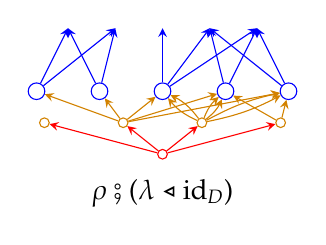
\begin{tikzpicture}
\node [rcol,vertex,small] (s) at (0, -8) {};
\coordinate (t1) at (-12,8) {};
\coordinate (t2) at (-6,8) {};
\coordinate (t3) at (-0,8) {};
\coordinate (t4) at (6,8) {};
\coordinate (t5) at (12,8) {};

\node [bcol,vertex] (m1_) at (-16,0) {};
\node [bcol,vertex] (m2_) at (-8,0) {};
\node [bcol,vertex] (m3_) at (0,0) {};
\node [bcol,vertex] (m4_) at (8,0) {};
\node [bcol,vertex] (m5_) at (16,0) {};

\node [ycol,vertex,small] (m1) at (-15,-4) {};
\node [ycol,vertex,small] (m2) at (-5,-4) {};
\node [ycol,vertex,small] (m3) at (5,-4) {};
\node [ycol,vertex,small] (m4) at (15,-4) {};

\draw [ycol,edge] (m2) -- (m1_);
\draw [ycol,edge] (m2) -- (m2_);
\draw [ycol,edge] (m2) -- (m3_);
\draw [ycol,edge] (m2) -- (m4_);
\draw [ycol,edge] (m2) -- (m5_);

\draw [ycol,edge,bend left=13] (m3) to (m3_);
\draw [ycol,edge,bend right=13] (m3) to (m3_);
\draw [ycol,edge,bend left=13] (m3) to (m4_);
\draw [ycol,edge,bend right=13] (m3) to (m4_);
\draw [ycol,edge,bend left=8] (m3) to (m5_);
\draw [ycol,edge,bend right=8] (m3) to (m5_);

\draw [ycol,edge] (m4) -- (m4_);
\draw [ycol,edge] (m4) -- (m5_);


\draw [rcol,edge] (s) -- (m1);
\draw [rcol,edge] (s) -- (m2);
\draw [rcol,edge] (s) -- (m3);
\draw [rcol,edge] (s) -- (m4);

\draw [bcol,edge] (m1_) -- (t1);
\draw [bcol,edge] (m1_) -- (t2);

\draw [bcol,edge] (m2_) -- (t1);
\draw [bcol,edge] (m2_) -- (t2);

\draw [bcol,edge] (m3_) -- (t3);
\draw [bcol,edge] (m3_) -- (t4);
\draw [bcol,edge] (m3_) -- (t5);

\draw [bcol,edge] (m4_) -- (t4);
\draw [bcol,edge] (m4_) -- (t5);

\draw [bcol,edge] (m5_) -- (t4);
\draw [bcol,edge] (m5_) -- (t5);


\node at (0, -13) {$\rho \fatsemi (\lambda \sub \id_D)$};
\end{tikzpicture}

    \quad
    $\canoniso$
    \quad
    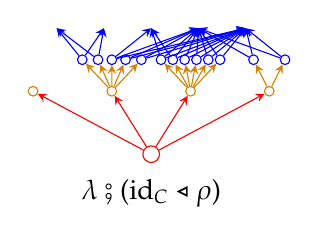
\begin{tikzpicture}
\node [rcol,vertex] (s) at (0, -8) {};
\coordinate (t1) at (-12,8) {};
\coordinate (t2) at (-6,8) {};
\coordinate (t3) at (0,8) {};
\coordinate (t4) at (6,8) {};
\coordinate (t5) at (12,8) {};

\node [ycol,vertex,small] (m1) at (-15,0) {};
\node [ycol,vertex,small] (m2) at (-5,0) {};
\node [ycol,vertex,small] (m3) at (5,0) {};
\node [ycol,vertex,small] (m4) at (15,0) {};

\node [bcol,vertex,small] (m21) at (-8.75,4) {};
\node [bcol,vertex,small] (m22) at (-6.75,4) {};
\node [bcol,vertex,small] (m23) at (-5,4) {};
\node [bcol,vertex,small] (m24) at (-3.25,4) {};
\node [bcol,vertex,small] (m25) at (-1.25,4) {};
\node [bcol,vertex,small] (m31) at (1.25,4) {};
\node [bcol,vertex,small] (m32) at (2.75,4) {};
\node [bcol,vertex,small] (m33) at (4.25,4) {};
\node [bcol,vertex,small] (m34) at (5.75,4) {};
\node [bcol,vertex,small] (m35) at (7.25,4) {};
\node [bcol,vertex,small] (m36) at (8.75,4) {};
\node [bcol,vertex,small] (m41) at (13,4) {};
\node [bcol,vertex,small] (m42) at (17,4) {};

\draw [rcol,edge] (s) -- (m1);
\draw [rcol,edge] (s) -- (m2);
\draw [rcol,edge] (s) -- (m3);
\draw [rcol,edge] (s) -- (m4);

\draw [ycol,edge] (m2) -- (m21);
\draw [ycol,edge] (m2) -- (m22);
\draw [ycol,edge] (m2) -- (m23);
\draw [ycol,edge] (m2) -- (m24);
\draw [ycol,edge] (m2) -- (m25);
\draw [ycol,edge] (m3) -- (m31);
\draw [ycol,edge] (m3) -- (m32);
\draw [ycol,edge] (m3) -- (m33);
\draw [ycol,edge] (m3) -- (m34);
\draw [ycol,edge] (m3) -- (m35);
\draw [ycol,edge] (m3) -- (m36);
\draw [ycol,edge] (m4) -- (m41);
\draw [ycol,edge] (m4) -- (m42);


\draw [bcol,edge] (m21) -- (t1);
\draw [bcol,edge] (m21) -- (t2);

\draw [bcol,edge] (m22) -- (t1);
\draw [bcol,edge] (m22) -- (t2);

\draw [bcol,edge] (m23) -- (t3);
\draw [bcol,edge] (m23) -- (t4);
\draw [bcol,edge] (m23) -- (t5);

\draw [bcol,edge] (m24) -- (t4);
\draw [bcol,edge] (m24) -- (t5);

\draw [bcol,edge] (m25) -- (t4);
\draw [bcol,edge] (m25) -- (t5);

\draw [bcol,edge] (m31) -- (t3);
\draw [bcol,edge] (m31) -- (t4);
\draw [bcol,edge] (m31) -- (t5);

\draw [bcol,edge] (m32) -- (t3);
\draw [bcol,edge] (m32) -- (t4);
\draw [bcol,edge] (m32) -- (t5);

\draw [bcol,edge] (m33) -- (t4);
\draw [bcol,edge] (m33) -- (t5);

\draw [bcol,edge] (m34) -- (t4);
\draw [bcol,edge] (m34) -- (t5);

\draw [bcol,edge] (m35) -- (t4);
\draw [bcol,edge] (m35) -- (t5);

\draw [bcol,edge] (m36) -- (t4);
\draw [bcol,edge] (m36) -- (t5);

\draw [bcol,edge] (m41) -- (t4);
\draw [bcol,edge] (m41) -- (t5);
\draw [bcol,edge] (m42) -- (t4);
\draw [bcol,edge] (m42) -- (t5);

\node at (0, -13) {$\lambda \fatsemi (\id_C \sub \rho)$};
\end{tikzpicture}

  \end{center}

  We will show that $M$ amounts to a profunctor\footnote{The notation
    $\cat{A} \prof \cat{B}$ for a profunctor
    $\cat{A}^\op \times \cat{B} \to \Set$ is due to Michael Shulman.}
  $(\int_{\cat{C}} X) \prof \cat{D}$, where $\cat{C}$ is the category
  corresponding to $C$, $X$ is a copresheaf on $\cat{C}$, and
  $\cat{D}$ is the category corresponding to $D$.

  Such a profunctor is the same as a prafunctor
  $\Set^{\cat{D}} \to \Set^{\cat{C}}$. Indeed,
  \begin{center}
    prafunctors $\Set^{\cat{D}} \to \Set^{\cat{C}}$
    
    $\updownarrow$
    
    \vspace{-.2em}\mbox{\phantom{\footnotesize for any $\cat{C}$-copresheaf $X$} right
      adjoint functors $\Set^{\cat{D}} \to \Set^{\cat{C}}/X$
      {\footnotesize for any $\cat{C}$-copresheaf $X$}}
    
    $\updownarrow$
    
    \vspace{-.2em}left adjoint functors $\Set^{\cat{C}}/X \to \Set^{\cat{D}}$
    
    $\updownarrow$
    
    \vspace{-.6em}left adjoint functors $\Set^{\int_{\cat{C}}X} \to \Set^{\cat{D}}$

    $\updownarrow$
    
    functors $(\int_{\cat{C}}X)^\op \to \Set^{\cat{D}}$

    $\updownarrow$

    profunctors $(\int_{\cat{C}} X) \prof \cat{D}$.
  \end{center}

  We have already seen that $M$ as a left $\cat{C}$-comodule amounts to a
  $\cat{C}$-copresheaf $X$ and a presheaf $Z$ on $\int_{\cat{C}}X$,
  and that $M$ as a right $\cat{D}$-comodule amounts to a family of
  $\cat{D}$-copresheaves $\{Z_i\}_{i \in I}$.

  The set $\pos{M}$ of positions in $M$ serves as both the set of
  elements in the $\cat{C}$-copresheaf $X$, that is,
  $\Ob(\int_{\cat{C}}X)$, as well as the indexing set $I$ for
  $\{Z_i\}_{i \in I}$. For any position $x \in \pos{M}$, the set
  $\dir{M}{x}$ of directions from $x$ serves as both $Z(x)$, the set of
  $x$-indexed elements in the $\int_{\cat{C}}X$-presheaf $Z$, as well
  as the set of elements in the $\cat{D}$-copresheaf $Z_x$.

  Moreover, $M$ and its left and right comodule structures are recovered
  from such information. That is, the data of a $\cat{C}$-copresheaf
  $X$, a $\int_{\cat{C}}X$-presheaf $Z$, and a $\cat{D}$-copresheaf
  structure on $Z(x)$ for each element $x$ in $X$ is the same as a
  polynomial $M$ equipped with the structure of a left
  $\cat{C}$-module and right $\cat{D}$-module, assuming no
  compatibility.

  The law $m(m(\atel{f}{x}, z), g) = m(\atel{f}{x}, m(z, g))$, encoding naturality
  of the maps $Z(\atel{f}{x}): Z(w) \to Z(x)$ (with respect to the
  $\cat{D}$-copresheaf structure on $Z(w)$ and $Z(x)$), is directly
  expressed by the bicomodule law, which identifies
  $\anydirmapof{\rho}{\anydirmapof{\lambda}{f \subd z} \subd g}$ with
  $\anydirmapof{\lambda}{f \subd \anydirmapof{\rho}{z \subd g}}$ whenever
  this makes sense.

  Thus, a bicomodule $M$ from $\cat{C}$ to $\cat{D}$ is the same as a
  functor $(\int_{\cat{C}} X)^\op \to \Set^{\cat{D}}$, i.e., a profunctor
  $(\int_{\cat{C}} X) \prof \cat{D}$ (i.e., a prafunctor from
  $\Set^{\cat{D}} \to \Set^{\cat{C}}$).
\end{proof}

\begin{prop}
  Maps between bicomodules are natural transformations between prafunctors.
\end{prop}
\begin{proof}
  First, we see what a natural transformation between prafunctors
  translates to under the correspondence between prafunctors and
  profunctors.

  Recall\footnote{We have not shown this in this paper.} that a
  prafunctor $\Set^{\cat{D}} \to \Set^{\cat{C}}$ is the same as a
  functor from $\cat{C}$ into the category of prafunctors
  $\Set^{\cat{D}} \to \Set$, and that prafunctors
  $\Set^{\cat{D}} \to \Set$ are coproducts of representables. Hence a
  prafunctor decomposes into a $\cat{C}$-shaped diagram of coproducts
  of representable functors $\Set^{\cat{D}} \to \Set$, and maps of
  prafunctors are maps of such diagrams. A natural transformation
  between such coproducts of representables
  \[\sum_{x \in X\!(c)}\Hom(Z_x, -) \quad \to \quad \sum_{x' \in X'\!(c)}\Hom(Z_{x'}',
    -)\] is the same as a function $\posmap{\alpha}$ from $X(c)$ to
  $X'(c)$ and a map of $\cat{D}$-presheaves
  ${Z_{\posmapof{\alpha}{x}} \to Z_x}$ for each $x \in X(c)$ (by the
  Yoneda lemma). On that account, we can see how a $\cat{C}$-shaped
  diagram of natural transformations is a $\cat{D}$-copresheaf-valued
  presheaf on the category of elements of a $\cat{C}$-copresheaf: the
  arrows of $\cat{C}$ act as functions between the indexing sets of
  $\cat{D}$-copresheaf families $\{Z_x\}_{x \in X(c)}$, and along each
  application of an arrow is a $\cat{D}$-copresheaf map in the
  opposite direction.

  Putting it all together, a natural transformation between
  prafunctors corresponding to profunctors
  $Z : (\int_{\cat{C}} X)^\op \to \Set^{\cat{D}}$ and
  $Z' : (\int_{\cat{C}} X')^\op \to \Set^{\cat{D}}$ (where $X$ and
  $X'$ are $\cat{C}$-copresheaves) amounts to a copresheaf map
  $\posmap{\alpha}$ from $X$ to $X'$ and maps $\dirmap{\alpha}{x}$
  from $Z'(\posmapof{\alpha}{x})(d)$ to $Z(x)(d)$, natural in $x$ and
  $d$. (Moreover, vertical composition of natural transformations
  between prafunctors corresponds to the evident composition of such
  $\alpha$ maps.)

  Let $C$ and $D$ be polynomial comonoids (with corresponding
  categories $\cat{C}$ and $\cat{D}$). Let $M$ and $N$ be bicomodules
  from $C$ to $D$, and let $\alpha$ be a bicomodule map from $M$ to
  $N$.

  As usual, $\alpha$ consists of maps
  $\posmap{\alpha}: \pos{C} \to \pos{D}$ and
  $\dirmap{\alpha}{x}: \dir{D}{\posmapof{\alpha}{x}} \to \dir{C}{x}$
  for all positions $x \in \pos{C}$. Translated into language about
  the corresponding profunctors, $\posmap{\alpha}$ is a map from the
  set of elements of $X_M$ to the set of elements of $X_N$ (where
  $X_M$ and $X_N$ are the $\cat{C}$-copresheaves induced by $M$ and
  $N$, respectively), and $\dirmap{\alpha}{x}$ is a map from
  $Z_N(\posmapof{\alpha}{x})$ to $Z_M(x)$ (where $Z_M$ and $Z_N$ are
  the $\int_{\cat{C}}X_M$-presheaf and $\int_{\cat{C}}X_N$-presheaf
  induced by $M$ and $N$, respectively).

  We verify this $\alpha$ corresponds to a natural transformation
  between prafunctors $\Set^{\cat{D}} \to \Set^{\cat{C}}$ in the sense
  described above.
  \begin{itemize}
  \item The naturality in $c$ law
    $\posmapof{\alpha}{m(x,f)} = m(\posmapof{\alpha}{x},f)$ for the
    $\cat{C}$-copresheaf map is the content of the left comodule map
    law
    $\alpha \fatsemi \lambda_N = \lambda_M \fatsemi (\id_C \sub
    \alpha)$ as regards positions.
    
    (This also forces the law $t(\posmapof{\alpha}{x}) = t(x)$, i.e.,
    $\posmap{\alpha}$ preserves indexing objects.)
  \item The law $t(\dirmapof{\alpha}{x}{z}) = t(z)$ (i.e.,
    $\dirmap{\alpha}{x}$ preserves indexing objects of elements)
    is the content of the right comodule map law
    $\alpha \fatsemi \rho_N = \rho_M \fatsemi (\alpha \sub \id_D)$ as
    regards positions.
  \item The naturality in $x$ law
    $\dirmapof{\alpha}{x}{m(\atel{f}{\posmapof{\alpha}{x}}, z)} =
    m(\atel{f}{x}, \dirmapof{\alpha}{m(x, f)}{z})$ is the content of the
    left comodule map as regards directions, which identifies
    ${\anydirmapof{\alpha}{\anydirmapof{\lambda_N}{f \subd z}}}$ with
    $\anydirmapof{\lambda_M}{f \subd \anydirmapof{\alpha}{z}}$ whenever
    this makes sense.
  \item The naturality in $d$ law
    $\dirmapof{\alpha}{x}{m(z, f)} = m(\dirmapof{\alpha}{x}{z}, f)$
    for the maps $\dirmap{\alpha}{x}$ as $\cat{D}$-copresheaf maps is
    the content of the right comodule map law as regards directions,
    which identifies
    $\anydirmapof{\alpha}{\anydirmapof{\rho_N}{z \subd f}}$ with
    $\anydirmapof{\rho_M}{\anydirmapof{\alpha}{z} \subd f}$ whenever
    this makes sense.
  \end{itemize}

  Conversely, any natural transformation between prafunctors
  $\Set^{\cat{D}} \to \Set^{\cat{C}}$ gives rise to such an $\alpha$,
  satisfying such laws.

  (Moreover, note that vertical compositions are preserved under the
  correspondence between prafunctor natural transformations and
  bicomodule maps, since vertical composition of such natural
  transformations is achieved by composing the $\alpha$ maps relating
  the underlying profunctors.)
\end{proof}

\begin{prop}
  Composition of bicomodules is composition of prafunctors.
\end{prop}
\begin{proof}
  Bicomodules from $D$ to $0$ specialize to copresheaves on $\cat{D}$
  (and maps between such bicomodules are copresheaf maps). Hence each
  bicomodule $M$ from $C$ to $D$ induces a functor $M^*$ from
  $\cat{D}$-copresheaves to $\cat{C}$-copresheaves by
  precomposition. Accordingly, we have
  $(M \sub_D N)^* \cong N^* \fatsemi M^*$ (where $M: C \bim D$ and
  $N: D \bim E$ are bicomodules).
  
  We show that the profunctor-induced prafunctor corresponding to the
  bicomodule $M$ is the same functor $M^*$ induced by horizontal
  precomposition of $M$.

  Recall\footnote{We have not shown this in this paper.} that the
  composite $M \sub_D N$ of bicomodules ${M: C \bim D}$ and
  ${N: D \bim E}$ is the equalizer of $\id_M \subd \lambda_N$ and
  $\rho_M \subd \id_N$. Its bicomodule structure is given by the
  unique transformations
  \[\lambda_{M \sub_D N}: M \sub_D N \to C \sub M \sub_D N \quad
    \text{ and } \quad \rho_{M \sub_D N} : M \sub_D N \to M \sub_D N
    \sub E\] such that
  \[\lambda_{M \sub_D N} \fatsemi (\id_C \sub \iota) = \iota \fatsemi
  (\lambda_M \sub \id_N) \quad \text{ and } \quad
  \rho_{M \sub_D N} \fatsemi (\iota \sub \id_E) = \iota \fatsemi
  (\id_M \sub \rho_N),\] where $\iota$ is the ``inclusion''
  $M \sub_D N \hookrightarrow M \sub N$.

  Concretely, the positions in $\pos{(M \sub_D N)}$ are the positions
  $a$ in $\pos{(M \sub N)}$ such that
  $\posmapof{(\id_M \sub \lambda_N)}{a} = \posmapof{(\rho_M \sub
    \id_N)}{a}$, and the directions in $\dir{(M \sub_D N)}{a}$ are the
  equivalence classes of directions in $\dir{(M \sub N)}{a}$ under the
  equivalence relation generated by
  \[\dirmapof{(\id_M \sub \lambda_N)}{a}{z_M \subd d \subd z_N} \sim \dirmapof{(\rho_M \sub
      \id_N)}{a}{z_M \subd d \subd z_N}\] for all directions
  $z_M \subd d \subd z_N$ from
  $\posmapof{(\id_M \sub \lambda_N)}{a} = \posmapof{(\rho_M \sub
    \id_N)}{a}$, i.e., we have
  \[z_M \subd \anydirmapof{\lambda_N}{d \subd z_N} \sim
    \anydirmapof{\rho_M}{z_M \subd d} \subd z_N\] whenever this makes
  sense. The transformations $\lambda_{M \sub_D N}$ and
  $\rho_{M \sub_D N}$ respectively agree with $\lambda_M \sub \id_N$
  and $\id_M \sub \rho_N$ on positions, and similarly they send
  directions $c \subd [z_M \subd z_N]$ to
  $[\anydirmapof{\lambda_M}{c \subd z_M} \subd z_N]$ and
  $[z_M \subd z_N] \subd e$ to
  $[z_M \subd \anydirmapof{\rho_M}{z_M \subd e}]$ whenever this makes
  sense. (As we will see, we will not end up needing to think about
  directions in $M \sub_D N$ at all.)

  We are interested in the case where $E = 0$. Here $\rho_N$ is
  trivial and $N$ is constant (just a set $\pos{N}$ of empty
  positions) with a $\cat{D}$-copresheaf structure induced by
  $\lambda_N$. As a right $D$-comodule, $M$ describes a family of
  $\cat{D}$-copresheaves. Hence $(- \sub_D -)$ may be viewed as an
  operation that takes as input a family of $\cat{D}$-copresheaves
  $\{Z_x\}_{x \in X}$ plus another $\cat{D}$-copresheaf $U$ and
  returns a constant polynomial $P$ (i.e., a set). The positions in
  $P$ are the $p \in \pos{(M \sub N)}$ such that
  $m(p_z, f) = p_{m(z, f)}$ for all $z \in M[p_\base]$. Such a $p$ is
  the same as a natural transformation from any one of the $Z_x$ to
  $U$.

  This set of natural transformations $P$ is endowed with a
  $\cat{C}$-copresheaf (left $C$-comodule) structure
  $\lambda_{M \sub_D N}$, induced by $\lambda_M$. Indeed, $\lambda_M$
  supplies a covariant action by $\cat{C}$ on the indexing set $X$ of
  $\{Z_x\}_{x \in X}$ and supplies a natural transformation
  $Z(\atel{f}{x}): Z_w \to Z_x$ whenever $x$ is sent to $w$ by
  $f \in \cat{C}$. So we obtain a covariant $\cat{C}$-action on the
  set of natural transformations from members of $\{Z_x\}_{x \in X}$
  to $U$ by precomposing such $Z(\atel{f}{x})$ maps.

  In summary,
  \[P(c) = (M^*(U))(c) = \sum_{x \in X\!(c)}\Hom_{\Set^\cat{D}}(Z_x, U).\]

  This characterizes the behavior of $M^*$ on objects. We see the
  expected form of the prafunctor corresponding to $M$. In particular,
  when $U$ is the terminal $\cat{D}$-copresheaf, $P$ is $X$ (the
  $\cat{C}$-copresheaf induced by $\lambda_M$).
  
  Next, we seek the behavior of $M^*$ on maps. Recall\footnote{We have
    not shown this in this paper.} that the horizontal composite
  $\alpha \sub_D \beta$ of bicomodule maps $\alpha: M \to M'$ and
  $\beta: N \to N'$ is the unique transformation
  $M \sub N \to M' \sub N'$ such that
  \[(\alpha \sub_D \beta) \fatsemi \iota_{M' \sub_D N'} = \iota_{M
      \sub_D N} \fatsemi (\alpha \sub \beta),\] where
  $\iota_{M \sub_D N}$ and $\iota_{M' \sub_D N'}$ are respectively the
  ``inclusions'' ${M \sub_D N \hookrightarrow M \sub N}$ and
  ${M' \sub_D N' \hookrightarrow M' \sub N'}$.

  Concretely, the transformation $\alpha \sub_D \beta$ agrees with
  $\alpha \sub \beta$ on positions, and similarly it sends directions
  $[z_{M'} \subd z_{N'}]$ to
  $[\anydirmapof{\alpha}{z_{M'}} \subd \anydirmapof{\beta}{z_{N'}}]$
  whenever this makes sense. (But again, we will not need to look at
  directions.)

  We will be taking $\alpha = \id_M$, i.e., horizontally precomposing
  the bicomodule $M$ with the map $\beta$. Since our $N, N': D \bim 0$
  are constant, $\beta$ is entirely detemined by the map of positions
  $\posmap{\beta}$, which amounts to a natural transformation between
  $\cat{D}$-copresheaves. Hence $M \sub_D \beta$ sends each position
  $a \in \pos{(M \sub_D N)} \subseteq \pos{(M \sub N)}$ to the
  position $a' \in \pos{(M \sub_D N')} \subseteq \pos{(M \sub N')}$
  such that ${a'}_\base = a_\base$ and
  ${a'}_z = \posmapof{\beta}{a_z}$ for all directions
  $z \in M[a_\base]$. In other words, it is the map that sends a
  natural transformation $p \in P = \pos{(M \sub_D N)}$ to
  $p \fatsemi \posmap{\beta}$. This characterizes the behavior of
  $M^*$ on maps (which could already have been anticipated based on
  the formula for $M^*(U)$ given above).

  The $\cat{C}$-copresheaf map $M^*(!_U)$ (where $!_U: U \to 1$)
  assigns each $p: Z_x \to U$ in $M^*(U)$ the index $x \in X$ of its
  domain $Z_x$, equipping $M^*U$ with the structure of a
  $\int_{\cat{C}}X$-copresheaf. This is the canonical lift of the
  functor $M^*: \Set^{\cat{D}} \to \Set^{\cat{C}}$ to a functor
  $\slicelift{M^*}: \Set^{\cat{D}} \to \Set^{\cat{C}}/M^*(1) =
  \Set^{\cat{C}}/X \cong \Set^{\int_{\cat{C}}X}$.

  It is left to observe that $\slicelift{M^*}$ is right adjoint to
  $\cocoextend{Z}: \Set^{\int_{\cat{C}}X} \to \Set^{\cat{D}}$, the
  cocontinuous extension of the functor
  $Z: (\int_{\cat{C}}X)^\op \to \Set^{\cat{D}}$ to the free
  cocompletion of its domain. Fortunately, $U \mapsto \Hom(Z(-),U)$ is
  precisely the formula for the right adjoint of the cocontinuous
  extension of a (co)presheaf-valued functor $Z$ to the cocompletion of
  its domain.
\end{proof}

\begin{prop}
  Horizontal composition of bicomodule maps is horizontal composition
  of natural transformations between prafunctors.
\end{prop}
\begin{proof}
  Each bicomodule map $\alpha: M \to M': C \to D$ induces a natural
  transformation $\alpha^*:M^* \to {M'}^*$ by horizontal ($\sub_D$)
  precomposition. Accordingly, we have that the natural transformation
  $(\alpha \sub_D \beta)^*: (M \sub_D N)^* \to (M' \sub_D N')^*$ is
  equal to the horizontal composite (as natural transformations) of
  $\beta^*$ and $\alpha^*$, from $N^* \fatsemi M^*$ to
  ${N'}^* \fatsemi {M'}^*$ (where both $\alpha: M \to M': C \bim D$
  and $\beta: N \to N': D \bim E$ are bicomodule maps).

  Let $N$ be a bicomodule $D \bim 0$ (i.e., a
  $\cat{D}$-copresheaf). The component of $\alpha^*: M^* \to {M'}^*$
  at $N$ is $\alpha \sub_D \id_N: M^*(N) \to {M'}^*(N)$. The map on
  positions $\posmap{(\alpha \sub_D \id_N)}$ agrees with
  $\posmap{(\alpha \sub \id_N)}$, and since $M' \sub_D N$ is constant,
  there are no directions to account for. This map
  $\posmap{(\alpha \sub_D \id_N)}$ sends each position
  ${a \in M \sub_D N \subseteq M \sub N}$ to the position
  ${a' \in M' \sub_D N \subseteq M' \sub N}$ such that
  ${a'}_\base = \posmapof{\alpha}{a_\base}$ and
  ${{a'}_z = a_{(\dirmapof{\alpha}{a_\base}{z})}}$ for all directions
  $z \in M'[\posmapof{\alpha}{a'_\base}]$.

  Recall $M \sub_D N$ is the $\cat{C}$-copresheaf
  $\sum_{x \in X\!(-)} \Hom(Z(x),U)$, where $Z$ is the functor
  $\int_{\cat{C}}X \to \Set^{\cat{D}}$ corresponding to $M$ and $U$ is
  the $\cat{D}$-copresheaf corresponding to $N$. We see that
  $\posmap{(\alpha \sub_D \id_N)}$ sends each ${p \in \Hom(Z(x),U)}$
  to
  $\dirmap{\alpha}{x} \fatsemi {p \in
    \Hom(Z(\posmapof{\alpha}{x}),U)}$. This is the relevant Yoneda
  embedding of $\dirmap{\alpha}{x}$, as a map of
  $\cat{D}$-copresheaves.

  Hence $\alpha^*$ is the same transformation of prafunctors derived
  from the data in $\alpha$, where indexes of $\cat{D}$-copresheaves
  are mapped according to $\posmap{\alpha}$ and elements are mapped
  backwards according to $\anydirmap{\alpha}$.
\end{proof}

\end{document}
